%-----------------------------------------------------------------
% WRITTEN BY: Matthias Ulbrich
% February 2017
%-----------------------------------------------------------------

\documentclass[12pt,a4paper]{scrartcl}				%KOMA-Skript

%\usepackage[ngerman]{babel}
\usepackage[USenglish]{babel}		%for separation rules, US for \DTMlangsetup
\usepackage[autostyle=true,german=quotes]{csquotes} %\enquote
\usepackage[utf8]{inputenc}			%fontencoding
\usepackage{hyperref}				%auto generate links in document
\usepackage{amsmath,amssymb,amsthm,mathtools}
\usepackage{color}					%\textcolor
\usepackage{acronym}				%abbreviations page
\usepackage{datetime2}		%\DTMlangsetup
\usepackage[margin=3.2cm]{geometry}
\usepackage{eucal}					%more calligraphy
\usepackage[nottoc]{tocbibind} 		%References in contents
\usepackage{svg}
\usepackage{graphicx}



\setcounter{tocdepth}{4}			%show subsubsubsections in table
\setcounter{secnumdepth}{4}
\DTMlangsetup{ord=raise}			%dates with superscript

\newcommand{\myparagraph}[1]{\paragraph{#1}\mbox{}\\} %paragraph with newline

%-----------------------------------------------------------------
% BEGIN DOCUMENT
%-----------------------------------------------------------------
\begin{document}

%-----------------------------------------------------------------
% TITLEPAGE
%-----------------------------------------------------------------
\begin{titlepage}

\begin{center}

\large
University of Bonn \\
Faculty of Mathematics and Natural Sciences \\
Institute of Computer Science IV \\
\vspace*{1 cm} 


\includegraphics[scale=0.11]{UniBonnSiegel.png}{\centering}
\vspace*{3 cm}  
    
{\fontfamily{cmss}\selectfont
	\Large
	Bachelor Thesis
	\vspace*{0.5cm}

	\LARGE 
	\textbf{A protocol for preserving the confidentiality of pailler-encrypted secrets while uncovering their homomorphic additions using secret sharing techniques}
	\vspace*{3 cm}       
}
  
Matthias Ulbrich \\  
2743974
\vspace{1 cm}

\today
\vspace*{1 cm}

\begin{tabular}{rl}
First examiner:  &Dipl.-Inf. Saffija Kasem-Madani \\
Second examiner: &Prof. Dr. Michael Meier
\end{tabular}

\end{center}
\end{titlepage}

%-----------------------------------------------------------------
% STATUTORY DECLARATION
%-----------------------------------------------------------------
\newpage
\pagenumbering{roman}

\section*{Statutory Declaration}

I hereby declare that I have authored this thesis independently, that I have not used other than the declared sources, and that I have explicitly marked all material which has been quoted either literally or by content from the used sources. \\[4ex]

Date: ....................      
\hspace*{1cm}
Signature: ..........................................
\clearpage

%-----------------------------------------------------------------
% NOTE OF THANKS AND DEDICATION
%-----------------------------------------------------------------
\section*{Note of thanks and dedication}

I want to thank my supervisor Dipl.-Inf. Saffija Kasem-Madani for the professional support and Prof. Dr. Michael Meier for the possibility to write this bachelor thesis in his department. \\
Many thanks to my girlfriend for the emotional support, to my sister, parents and my great aunt for the financial support during the course of my study. I dedicate this work to you.
\clearpage

%-----------------------------------------------------------------
% ABBREVIATIONS
%-----------------------------------------------------------------
\section*{Abbreviations}
During their first use these terms will be spelled out completely. Any further mentions will use the corresponding abbreviation.

\begin{acronym}[AAAA] 							% AAAA for alignment
	\acro{HBC}{Honest-but-curious}
	\acro{SMC}{Secure multi-party computation}
	\acro{SS}{Secret sharing}
	\acro{SSS}{Shamir's secret sharing}
	\acro{TTP}{Trusted third party}
\end{acronym}
\clearpage

%-----------------------------------------------------------------
% TABLE OF CONTENTS and LIST OF FIGURES
%-----------------------------------------------------------------
\tableofcontents
\listoffigures

%-----------------------------------------------------------------
%-----------------------------------------------------------------
%-----------------------------------------------------------------
% TEXT START
%-----------------------------------------------------------------
%-----------------------------------------------------------------
%-----------------------------------------------------------------
\newpage

\pagenumbering{arabic}
\setcounter{page}{1}				% start to count from 1

\section{Introduction}

Tracking of has become an omnipresent phenomenon in today's web. Common websites make use of multiple trackers  and these trackers communicate to third party services such as facebook \cite{HowOnlin70}. With constant tracking of users the accumulated data has to be stored and managed in a privacy-preserving manner. The german lawmaker calls to limit the use of personalized tracking data and encourages the use of methods of anonymization and pseudonymization in the Bundesdatenschutzgesetz \cite{BDSGEinz5}:

\begin{quote}
	\textbf{§3a Data reduction and data economy }\\
	The collection, processing and use of personal data and the selection and design of data processing systems must be geared to the goal of collecting, processing or using as little personal data as possible. In particular, personal data shall be anonymised or pseudonymized, insofar as this is possible according to the intended use and does not require disproportionate expenditure in relation to the intended protection purpose.\ (Translation by Google Translate\footnote{\url{translate.google.de},
		for the official translation: \url{www.gesetze-im-internet.de/englisch_bdsg}})
\end{quote}

 Many companies have build their business around tracking users around the web and evaluating their activities and preferences. Most well known are Google and Facebook which caused most of the third party requests in a 1-million-site census \cite{englehardt2016online}. Both companies which have made news when changing their terms of use for their services to be more privacy evasive or, in the case or Facebook when they aquire another company such as Instagram or WhatsApp. People fear for their privacy which seems at times out of control while at the same time law makers try to give indiviuals back control of their data \cite{NeueEUDa50}.

Laws makers call upon companies to anonymize data, which could very well also be in a companies interest for fear of public haze following hacking attempts of their publicized databases. Moreover, the accumulated data represents a value in itself upon which extended data-mining is performed to learn about users. Thus, it is evident that it is in a companies own interest to keep its data confidential even when sharing it with other parties.

In this thesis a design is proposed which allows a Data Holder - the party which originally accomulated tracking data - to share its information in such a way that analysis can be peformed without revealing the indivitual pieces of information in the database. Specificly, the database consists of positive integers (e.g. net income). The client (which will be referred to as the Analyzer from here on) is able to determine the total income of several individuals without gaining knowledge about the specific income of an individual in the process.

The design employs \textbf{s}hamir's \textbf{s}ecret \textbf{s}haring, an application of \textbf{s}ecure \textbf{m}ulti-party \textbf{c}omputation to achieve this. While determing the total of a subset of individuals net income does not directly reveal an individuals income, it is shown that by design allowing the computation of a very small subset can enable an attacker to end up gaining insight about individual data.


\section{Perequisites}

\subsection{Secure multi-party computation}
In an everyday context there are scenarios where competing parties may need to collude in computing. Take two millionares for example which want to know which one is richer without revealing their wealth to each other. This is known as the Millionaire's Problem and Andrew C. Yao has introduced a privacy-preserving SMC protocol for this problem in \cite{yao1982protocols}. Another example explained by Anna Lysyanskaya is how three parties can compute their net wight without having to admit their own weight to each other \cite{lysyanskaya2008keep}.

The most basic example is the use of a \textbf{t}rusted \textbf{t}hird \textbf{p}arty. All parties send their inputs to that party which computes and then returns the outcome to all parties. However, in the case of rivals privacy of the inputs is a main concern. A TTP is to be avoided and removed entirely from the protocol. This is where SMC comes in. SMC, also referred to as secure function evaluation is a term used in cryptography for designs which involve the participation of several parties to compute in conjunction over a distributed network - each party using their input - while keeping said input private towards the other parties. Thus, SMC enables parties with conflicting interest to cooperate with each other. 

Any design of a protocol will need to satisfy different constraints, one the one hand security constraints to make it secure against a to be defined attacker model and privacy constraints on the other hand, i.e. privacy guarantees which we want to supply with the protocol. Depending on the model of the attacker the design will differ to account for powers of the attacker. Thus any design needs to describe what security model it has taken into consideration for an outsider to know what it means when one is speaking of a secure design. We will discuss the types of various security models in \ref{sec:Security_models}.

Formally, an instance of a SMC problem can be defined as follows \cite[p.6]{Cramer}:
%https://en.wikibooks.org/wiki/LaTeX/Theorems
\newtheorem{mydef}{Definition}
\label{SMC}
\begin{mydef}
	\textbf{(Secure multi-party computation)}\\
	Given $n$ participating parties $P_1,P_2,...,P_n$ which each have a secret input $x_i$, these parties want to compute a function
	\begin{equation*}
	f(x_1,x_2,...,x_n)=y
	\end{equation*}
	jointly while satisfing the two conditions:
	\begin{enumerate}
		\item Input privacy: Party $P_i$ does not learn anything about $x_j$ for all $i\neq j$ during the execution of the protocol, i.e. there is no leakage of private data.
		\item Correctness: The function $f$ is correctly evaluated.
	\end{enumerate}
	When computing $f$ with regards to these two conditions we say that $f$ is computed \textit{securely}. Hence the name alternative name secure function evaluation.
\end{mydef}

Now an example of SMC: Computing the net weight of three individuals as mentioned by Lysyanskaya in \cite{lysyanskaya2008keep}. Alice has the input $x_1=45$, Bob the input $x_2=60$, and Carol the input $x_2=53$. These numbers refer to their weight in kilogram. How do they collude to determine their net weight? We want to evaluate the function $f(x_1,x_2,x_3)=\sum_i x_i$. In the proposed protocol each party firstly creates three random shares such that their sum equals their own weight mod $1000$. These shares are then distributed to the other parties. From then on Alice, Bob and Carol need to compute in conjunction to evalute the function $f$.

\begin{enumerate}
	\item Each party creates random shares depending on their input\\
	Alice: $(\textcolor{red}{140,620,285})$\\
	Bob: $(\textcolor{blue}{500,440,120})$\\
	Carol: $(\textcolor{green}{333,621,99})$
	\item Each party distributes two of their shares to the other parties.
	\item Each party adds these shares: \\
	Alice: $\textcolor{red}{140}+\textcolor{blue}{440}+\textcolor{green}{621}=_{1000} 201$\\
	Bob: $\textcolor{blue}{500}+\textcolor{red}{620}+\textcolor{green}{99}=_{1000} 219$ \\
	Carol: $\textcolor{green}{333}+\textcolor{red}{285}+\textcolor{blue}{120}=_{1000} 738$
	\item Each party broadcasts their result. 
	\item The sum mod 1000 of these values is the net weight of Alice, Bob and Carol. Everyone computes: $201+219+738=_{1000} 158$ $(=45+60+53)!$
\end{enumerate}

As we can see, this SMC protocoll enables Alice, Bob and Carol to compute their net weight correctly without giving up privacy. So both conditions mentioned in \ref{SMC} have been met. This functionality does come at a cost however, which is that the obfuscation by the computation is usually complex and requires more communication between the parties as can be seen in the example above. Computing the total weight of the tree parties requires five steps in total of which two steps require each party to communicate with all other parties. Thus, during the evaluation of the proposed design sheme of this thesis we will also take a look at common performace characterisitcs.

Is it also important to notice that in the example Alice, Bob and Coral were following the protocol and publishing the correct interim results in step four. Here it would be possible for an adversary to publish an incorrect interim result. Imagine for Coral to publish the value $748$ instead of $738$. Then Coral would still be able to perform the final calculation in private. But Alice and Bob are left in the dark about their true net weight. Both will assume that $168$ is their true net weight. However, while they have published their shares in step 2, they have not published their personal weights. We introduce the different types of adversaries in \ref{sec:Security_models}.

While the example is simple, the complexity of the communication may suggest that MPC is not entirely possible for any desired function. It has been shown that \textit{any} function can be securely evaluated. However, we need to assume that the majority of players is honest \cite{goldreich1987play}. To better describe how secure a SMC design is we will to introduce security models.

\subsection{Security models}
\label{sec:Security_models}

It is necessary to consider a security model which will underlie the design because the security model determines goals which are to be realized. A model is then called secure, if those security goals are met.  

\subsubsection{Honest-but-curious/passive adversary}
A honest-but-curious adversary, also referred to as a passive adversary follows the SMC protocol but is interested in breaking the privacy of other parties \cite{cramer2009}. An HBC adversay will try to extract as much information as possible from the given data, but cannot collude with other parties as this would deviate from the protocol. In that sense this can be considered a weak security model, if the parties in real world have an active interest in cooperating outside the protocol specifications to extract more information.

In Samim's thesis \cite{BASamim} an HBC adversary can leak the private data of a Pailler ciphertext by adding a zero which merely deforms the ciphertext. The Decrypter is not able to expose such an attack:
\begin{equation*}
Pailler_{k_p}(m)\ast Pailler_{k_p}(0)=Pailler_{k_0}(m+0)=Pailler^{\textcolor{red}{'}}_{k_p}(m)
\end{equation*}

\subsubsection{Malicious adversary}
Malicious adversaries don't follow the protocol specification and thus can collude with each other in order to subvert the privacy of another party.\cite{cramer2009} The SMC design will have to take into consideration any subset of parties that may act malicious (see \ref{AS}). Since a malicious adversary can deviate from the protocol he can send corrupt data or no data in particular to hinder other parties from computing the desired function as shown in the computation example earlier.

If $n$ denotes the number of parties participating in the protocol, it is possible to securely evalute any function for up to $t<n/2$ HBC adversaries (i.e. honest majority). In the case of malicious adversaries we can also tolerate up $t<n/2$ malicious adversaries, but the security is based on a computational assumption. \cite{smart2003}\cite[p.220]{goldreich1987play}.

\subsubsection{Static and dynamic adversary}
Both the HBC and Malicious adversaries may be static, meaning that from the beginning of the execution of the protocol up until the end no new parties are corrupted. However, to model a more agressive scenario it should be possible for an attacker that controls a participating party to infiltrate others during the execution. The dynamic adversary may, at any time, corrupt new players. This model is also referred to as adaptive security. \cite[p.79]{Cramer}.

The static malicious adversary is a fit model in cases where a party has been corrupted throught the whole process while a dynamic adversary is the most open model which takes into account any real word possibility. \cite{smart2003}

\subsubsection{Adversary structure}
\label{AS}
When considering a dynamic adversary it does not make sense to consider that \textit{any} amount of players can be corrupted (extreme case: all players are corrupted). There needs to be an honest majority to be able to design a secure SMC scheme as mentioned earlier. To limit the amount of parties that can be corrupted the term adversary structure is introduced \cite{cramer2009}: 

The adversary structure $\mathcal{A}$ is a family of subsets of the players limited in size:
\begin{enumerate}
	 \item If $(A\in \mathcal{A}) \wedge  (B\subset A) \Longrightarrow B\in \mathcal{A}$  (monotone)
	 
	 \item $\forall A\in \mathcal{A}: |A|<t$ (threshold)
\end{enumerate}

\subsubsection{Fair vs unfair}
\label{FU}
With asynchronous communication, one party may go last in order to subvert the protocol. This could be the case with Carol in step four of the aforementioned protocol example. Now Carol can subvert the protocol by not sending her interim result.

If a protocol ensures that \textit{all} players can still determine the correct evaluation or \textit{none} at all, we is called fair. \cite[p.386]{smart2003}

\subsubsection{Ideal-real-world model}
%https://en.wikipedia.org/wiki/Secure_multi-party_computation#Security_definitions
SMC is hard to formalize which is a problem, because the depicted problem is very general. Thus SMC was introduced in with two requirements in mind: Privacy of inputs and a correct result. However, this lax definition is not very formal and does not immediately lead to a definition of when a function has been securely evaluated. To measure security the ideal-real-word model is used \cite{cramer2009, CZ}:

A protocol is called secure if the adversary $\mathcal{A}$ does not \textit{learn more} in the real world than it would in the ideal world. 

Given a function $f$ we imagine an ideal, incorruptible implementation of $f$ in the functional $\mathcal{F}^f_{SFE}$ which leaks no private information. Then we achieve security by establishing a secure channel between the parties $P_i$ and $\mathcal{F}^f_{SFE}$. However, in the real word $f$ is implemented by some functional $\pi^f_{SFE}$. This functional needs to provide a protocol without the help of a TTP and with adversaries in mind. 

If we denote what the adversary $\mathcal{A}$ learns in the real word with $\text{IDEAL}_{\mathcal{A}}(\mathcal{F}^f_{SFE})$ and analogous $\text{REAL}_{\mathcal{A}}(\pi^f_{SFE})$ for what the adversary learns in the real world, we call the protocol $\mathcal{F}^f_{SFE}$ perfectly secure if
\begin{equation*}
\text{IDEAL}_{\mathcal{A}}(\mathcal{F}^f_{SFE}) = \text{REAL}_{\mathcal{A}}(\pi^f_{SFE})
\end{equation*}
%-----------------------------------------------------------------
% The latter may need some work. The sources cramer2009 and CZ 
% mentioned simulations.
%-----------------------------------------------------------------

\subsection{Secret sharing}
In the following section we will introduce the secret sharing paradigm using a method first described by Shamir \cite{shamir1979share}. Generall there secret sharing schemes fall into two categories: Yao's garbled circuit approach enables two-party SMC for his millionaire problem \cite{yao1982protocols}. \textbf{S}hamir's \textbf{s}ecret \textbf{s}haring enables SMC in a distributed network of two or more parties.
\subsubsection{Shamir's secret sharing}
\label{SSS}
Shamir's secret sharing is based on polynomials over a finite field $\mathbb{F}$, say $\mathbb{F}=\mathbb{Z}_p$ for some prime $p$.
Shamir's secrets sharing devides a numerical secret $s\in\mathbb{Z}_p$ using a polynomial $f(x)$ into $n$ \textit{unique} pieces of information which are called shares. When diving up a polynomial, these shares are evaluated function values $s_i \coloneqq f(i)$, i.e. $(i,s_i))$ are points on the graph of the polynomial function. These $s_i$ are divided among a set of $n$ shareholders identified by the index $i$. 

Any subset of k shareholders out of n can reconstruct the polynomial as a polynomial of degree $n-1$ is determined by n unique points. This is called a $(k,n)-threshold$ sharing sheme. 

Formally we define in accordance with Shamir\cite{shamir1979share}:

\newtheorem{KNSS}{Definition}
\begin{KNSS}
	(k,n) threshold sheme\\
	A (k,n) threshold sheme is a division of a piece of information D (e.g. a secret key) into n pieces $D_1,D_2,\ldots,D_n$ such that:
	\begin{enumerate}
		\item knowing any subset of $k$ pieces $D_i$ makes D easily computable
		\item knowing any subset of less than $k$ pieces $D_i$ leaves D undetermind in such a way that all possible values are equally likely
	\end{enumerate}
\end{KNSS}
\myparagraph{Sharing the secret}
Now imagine we have a secret $s\in\mathbb{Z}_p$. This numerical value is information which some data holder has collected. The data holder wants to sell this information for analysis while hiding the secret value. The data holder decides to employ a $(k,n)$ threshold scheme. In order to do so the data holder generates random coefficients $f_i\in\mathbb{F}_q$ with $i=1,\ldots,k$ and $k<n$ to form a random polynomial $f(x)$. Then k shares determine the polynomial. Note that the secret $s$ is selected to be the value of the polynomial when evaluated at zero $s=f(0)$:
\begin{equation*}
f(x)=s+f_1 x+f_2 x^2+\ldots+f_{k-1} x^{k-1}
\end{equation*}
The data holder has the role of a honest dealer when generating the shares from the polynomial. Set $X\subset\mathbb{F}_q\{0\}$, then the dataholder generates a random share by drawing a point from the polynomial for values $i\in X$. The zero value is excluded as the evaluation of the polynomial at zero is reserved to store the secret $s$. Finally, we end up with the vector:
\begin{equation*}
\text{Shares of s:}\ (s_1,\ldots,s_n)
\end{equation*}
Threshold sharing is enabled by generating equal or more shares than the degree of the polynomial, such that the points $(i,s_i)$ (over-)determine the polynomial.
%-----------------------------------------------------------------
% Bild einfügen
%-----------------------------------------------------------------

\myparagraph{Reconstructing the secret from k shares}
Now that the data holder has given out the shares, k shareholders can collude in reconstructing the polynomial and thus determine the secret. Given k shares $(s_1,\ldots,s_k)$ we want to reconstruct the secret $s$. This is accomplished by determining the Lagrange interpolation of $f(x)$:
\begin{equation*}
f(x)\coloneqq \sum_{i=0}^{k} \delta_{x_i}(x) f(x_i)
\end{equation*}
Where $\delta_{x_i}(x)$ is the Langrage basis polynomial defined as:
\begin{equation*}
\delta_{x_i}(x)\coloneqq \prod_{i\neq j} (x-x_j)(x_i-x_j)^{-1}
\end{equation*}
The left factor guarantees that the langrange polynomial evaluates to $1$

% for all of SSS
\cite{smart2003}

\subsubsection{Homomorphic Secret Sharing}
Homomorphic Secret Sharing refers to a secret sharing sheme which employs an operation $\otimes$ on the shares \cite{schoenmakers1999simple}. The combination of secret shares then enables to reconstruct a polynomial for the under $\otimes$ \textit{combined} secrets. Formally, we define the homophoric property of a sharing sheme as introduced by \cite{benaloh1986secret}.


\newtheorem{HSS}{Definition}
\begin{HSS}$(\otimes,\oplus)$-homomorphic \\
	Given the operators $\otimes$ on the secret domain T and $\oplus$ on share domain S, a (k,n) threshold sheme is called $(\otimes,\oplus)$-homomorphic if for all functions $F_I:T^k\rightarrow S$ which compute the secret value of the secret sharing mechanism the follow implication is valid:
	
	\begin{align*}
						D  &= F_I(D_{i_1},D_{i_2},\ldots,D_{i_k})\quad  \wedge \\
						D' &= F_I(D'_{i_1},D'_{i_2},\ldots,D'_{i_k}) \\
		\Rightarrow	D\otimes D' &= F_I(D_{i_1}\oplus D'_{i_1},D{i_2}\oplus D'_{i_2},\ldots,D_{i_k}\oplus D'_{i_k})
	\end{align*}
	
\end{HSS}

Shamir's Secret Sharing as described in \ref{SSS} is $(+,+)$-homomorphic. This property will be used in our design proposed in \ref{Design}.

\subsubsection{Verifiable Secret Sharing}
A key tool for secure MPC, interesting in its own right, is verifiable secret sharing (VSS):
a dealer distributes a secret value s among the players, where the dealer and/or some of
the players may be cheating. It is guaranteed that if the dealer is honest, then the cheaters
obtain no information about s, and all honest players are later able to reconstruct s, even
against the actions of cheating players. Even if the dealer cheats, a unique such value s will
be determined already at distribution time, and again this value is reconstructable even
against the actions of the cheaters.\cite{cramer2009}

\begin{figure}[ht]
	\centering
	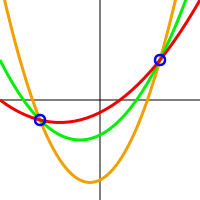
\includegraphics[scale=0.3]{test}
	\caption{Ein Testbild}
\end{figure}

%% MALLEABILITY
\subsection{The Pailler Cryptosystem}

\subsubsection{Encryption}
% with key generation

\subsubsection{Decryption}

\subsubsection{Homomorphic properties}

\subsubsection{Malleability}

\section{A protocol for SMC with SSS}
\label{Design}

\subsection{Related work}
\subsection{Design}
\subsubsection{Dealer}
\subsubsection{Analyzer}
\subsubsection{Shareholder}

\subsection{Implementation of the Protocol}
%vgl. Paper aus Darmstadt für Darstellung
\subsubsection{Dealer}
\subsubsection{Analyzer}
\subsubsection{Shareholder}

\subsection{Evaluation of the Protocol}
\subsubsection{Input Privacy and Correctness}
\subsubsection{Ideal-real-world comparison}
\subsubsection{A differential attack}

\subsection{Final words}





In this chapter a design is proposed which allow a user to ga...
Assumtion made: Secure channels, and identification of other users: TLS with signatures.
The shares shares distributed by the dataholder are consistent. VSS



Sonstige: Stichwörter
provably secure
semi-honest
privacy-preserving
perfect security
%Formal definition SS 267


%-----------------------------------------------------------------
% BIBLIOGRAPHY
%-----------------------------------------------------------------
\newpage

\small
\bibliographystyle{alpha}				% Name+Year instead of numbers
\bibliography{Literaturverzeichnis}		% Literaturverzeichnis.bib

\end{document}





